\documentclass[../main.tex]{subfiles}

\begin{document}

% -----------------------
% Definición del concepto
% -----------------------
\subsubsection{Definición del concepto.}
% \cite{EvaluationFramework},  \cite{ionnetwork},
Una primera manera de concebir la \acrfull{SSI} como alternativa a la tradicional manera de gestión de credenciales es percatándonos del papel que el propio usuario tiene tras el establecimiento de este paradigma. Mientras que normalmente no disponían de métodos que de manera autónoma pudieran identificarlos, haciéndolos dependientes de una tercera parte, ahora acceden a los diferentes servicios identificándose ellos mismos mediante credenciales autogestionadas en sus carteras digitales.
\\

Encontramos definiciones similares en esta misma línea leyendo la literatura, como es el caso de \cite{EvaluationFramework} donde se nos muestra que ``la Identidad Autosoberana es una representación digital de las características, descripciones e identificadores de los individuos donde ningún gobierno u organización puede violar nuestro derecho a elegir nuestro nivel de privacidad o grado de visibilidad con nuestros atributos de identidad.''
\\

\begin{figure}[htbp]
    \centering
    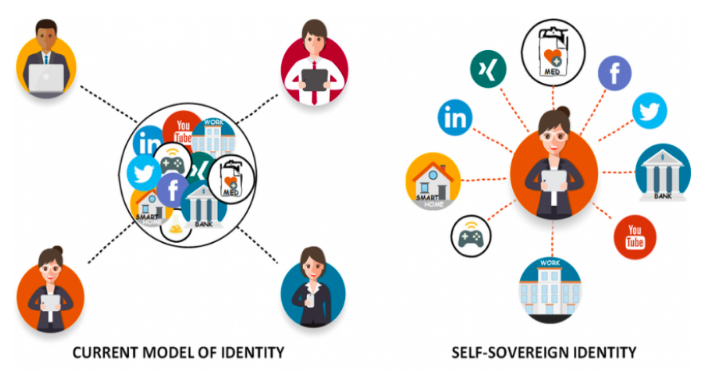
\includegraphics[width=0.75\linewidth]{images/SSI_vs_Traditional.png}
    \caption{\textit{Comparativa entre ambos paradigmas.} Fuente \cite{DefSSI}}
    \label{fig:comparacion}
\end{figure}

Este radical cambio necesariamente requiere redefinir aspectos clave como la función que desempeñan los diferentes \hyperref[Actores y sus funciones en el paradigma]{actores} y la propia \hyperref[Arquitectura y marco de referencia]{arquitectura} de sus componentes, además de dotar con \hyperref[Carteras de Identidad Digital]{medios técnicos} a los usuarios.


% ---------------------------------------
% Actores y sus funciones en el paradigma
% ---------------------------------------
\newpage
\subsubsection{Actores y sus funciones en el paradigma.}\label{Actores y sus funciones en el paradigma}
Tal y como se detalla en \cite{ChallengesSSI}, nos encontramos en un escenario con tres principales actores:

\begin{itemize}
    \item \textbf{Emisor} (Issuer). Responsable de \textbf{generar} las credenciales pedidas por los usuarios. 
    \\ Pueden ser entidades gubernamentales, corporaciones e incluso individuos.
    
    \item \textbf{Titular} (Holder). Es el usuario propiamente dicho, el cual \textbf{dispone} de sus credenciales expedidas por el emisor y las almacena en su Cartera de Identidad Digital. 
     \\ Representa a todo aquel portador de Identidad Digital, de cualquier naturaleza.
    
    \item \textbf{Verificador} (Verifier). Recibe y procesa las credenciales para \textbf{verificar} su validez. 
    \\ Representan a aquellos interesados en comprobar la identidad de los Titulares, como pueden ser las instituciones o los negocios. 
    \\
\end{itemize}

\begin{figure}[htbp]
    \centering
    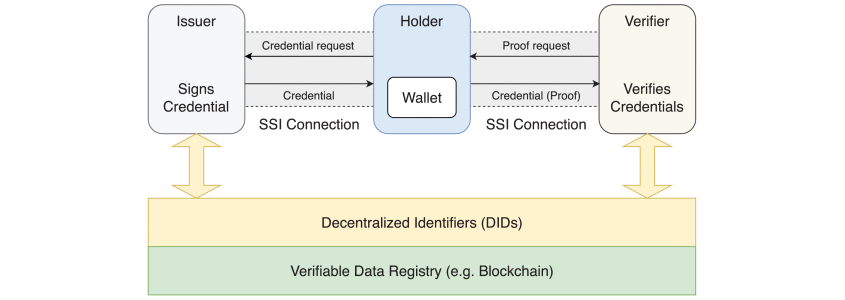
\includegraphics[width=1\linewidth]{images/ActoresSSI.png}
    \caption{\textit{Principales actores de la \acrshort{SSI} y sus comunicaciones.} Fuente \cite{ChallengesSSI}}
    \label{fig:actoresSSI}
\end{figure}

\refstepcounter{observacion}
\begin{tcolorbox}[colback=gray!10!white, colframe=gray!50!black, title=Observación \theobservacion]\label{observacion-actores}
Es importante destacar que se mediante este esquema se desacopla la emisión y verificación de credenciales, del registro de estas. De esta manera se permite desplegar los \acrshort{DID}s sobre una blockchain o sobre un repositorio centralizado indistintamente. 
\end{tcolorbox}


% ----------------------------------
% Arquitectura y marco de referencia
% ----------------------------------
\newpage
\subsubsection{Arquitectura y marco de referencia.}\label{Arquitectura y marco de referencia}
También en \cite{ChallengesSSI} se elabora una \textbf{arquitectura multicapa} con el objetivo de estandarizar e ``integrar la tecnología con la responsabilidad humana en todas las capas legales y sociales''. \\
Destacar que existen diversos marcos de referencia expuestos en numerosos artículos académicos, pero se decide destacar este en concreto ya que realiza una división en pilas (stacks) para estructurar sus componentes, los cuales varían entre \textbf{fundamentos técnicos} en capas inferiores y \textbf{protocolos} en las superiores.
\\

\begin{figure}[htbp]
    \centering
    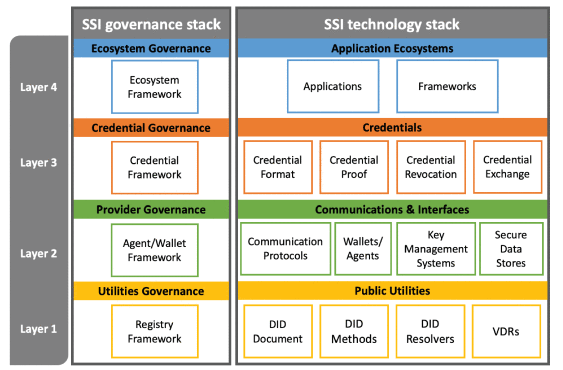
\includegraphics[width=0.75\linewidth]{images/ArquitecturaSSI.png}
    \caption{\textit{Arquitectura multi-stack para la \acrshort{SSI}.} Fuente \cite{ChallengesSSI}}
    \label{fig:ArquitecturaSSI}
\end{figure}

Esta arquitectura propuesta resulta interesante porque tiene en cuenta esta \textbf{dualidad} en el paradigma, siendo de gran utilidad en \hyperref[Riesgos y amenazas]{secciones posteriores}. Además, aunque no se entra a describirla en profundidad en este \acrshort{TFG}, nos ayuda a comprender con mayor facilidad los fundamentos técnicos sobre los que se sustenta. 

En la misma línea, se recomienda la lectura de \cite{EvaluationFramework} en la que se propone un marco de evaluación para los sistemas de la \acrshort{SSI} y se realiza un análisis aplicándolo a uPort, Sovrin, ShoCard, Civic y Blockstack, las cuales representan diferentes \textbf{implementaciones} de este paradigma. 


% -----------------------------
% Carteras de Identidad Digital
% -----------------------------
\newpage
A continuación, se detallaran las tecnologías que permiten que este paradigma sea factible. La principal fuente de información de esta sección es \acrfull{W3C}, aunque será complementada por otras alternativas en determinadas subsecciones.

A fecha de la elaboración de este escrito, las versiones más actualizadas corresponden a ``Decentralized Identifiers (DIDs) v1.0'' \cite{DID-core} y ``Verifiable Credentials Data Model v2.0'' \cite{VC-data-model}.
\\

\subsubsection{Carteras de Identidad Digital.}\label{Carteras de Identidad Digital}
Seguramente sea el componente mayormente reconocido del paradigma, debido a que resulta familiar al usuario (paralelismo con la cartera física) y es de uso generalizado en otras tecnologías como las \Gls{criptodivisas} o métodos de pago alternativos como Google Wallet. 

Sin embargo, esta cartera `genérica' debe ser adaptada al paradigma para que sea capaz de ``firmar, cifrar, reenviar mensajes relacionados con credenciales y establecer conexiones de agente a agente'' \cite{ChallengesSSI}, además de permitir el almacenamiento de las propias credenciales.
\\

\refstepcounter{observacion}
\begin{tcolorbox}[colback=gray!10!white, colframe=gray!50!black, title=Observación \theobservacion]\label{observacion-cartera}
El hecho de que una Cartera Digital (o solución que la implemente) pueda almacenar documentos identificativos como pasaportes, DNIs o similares \textbf{NO} quiere decir que sea una Cartera de Identidad Digital, al menos no como la concebimos en este escrito. 
\\ Recordar que deben cumplirse los requisitos técnicos que garanticen la descentralización e implementación de funcionalidades del paradigma de la \acrshort{SSI}, entre otros aspectos. 
\end{tcolorbox}
\newpage


% --------------------------------
% Identificadores Descentralizados
% --------------------------------
\newpage
\subsubsection{Identificadores Descentralizados.}\label{Identificadores Descentralizados}
Como hemos visto anteriormente, la base técnica sobre la que se sustenta el paradigma es el \acrfull{DID}. Estos siguen el formato de un \Gls{URI} y están compuestos por tres elementos:

\begin{itemize}
    \item \textbf{Esquema} (\textcolor{blue}{Scheme}). \\
    Definido como `did', representa al esquema de identificación a seguir.
    
    \item \textbf{Método DID} (\textcolor{purple}{DID Method}). \\
    Indica la manera de realizar la resolución del \acrshort{DID}s. Destacar que algunas de estas implementaciones fueron ya mencionadas en \ref{Arquitectura y marco de referencia}. Por ejemplo, `sov' correponde a Sovrin.
    
    \item \textbf{Identificador Específico} (\textcolor{teal}{Specific Identifier}). \\ 
    Permite asociar inequívocamente al usuario dentro del método en cuestión, al ser único.
\end{itemize}

\begin{figure}[htbp]
    \centering
    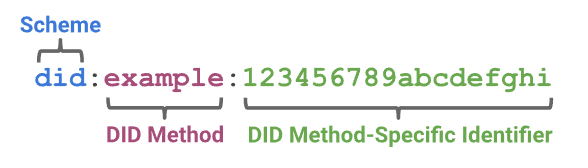
\includegraphics[width=0.75\linewidth]{images/DID_Estructura.png}
    \caption{\textit{Estructura genérica de un \acrshort{DID}.} Fuente \cite{DID-core}}
    \label{fig:DID_Estructura}
\end{figure}

A continuación, definiremos el resto de componentes que conforman la arquitectura sin entrar en profundidad en los detalles concretos de la implementación, como los parámetros que poseen o interfaces disponibles.  

\begin{itemize}
    \item \textbf{URL DID} (DID URL). \\
    Son una extensión sintáctica de los \acrshort{DID} y permite la referenciación a recursos internos o externos. Siguiendo el ejemplo, \textit{did:example:123456789abcdefghi/path/to/rsrc} busca en el directorio descrito un archivo del paradigma, como los \underline{Documentos DID}. 
    
    \item \textbf{Documento DID} (DID Document). \\
    Es una representación de la información que describe a un \underline{Sujeto DID}, el cual está siendo identificado mediante su \acrshort{DID}, incluyendo mecanismos como las claves públicas.
    
    \item \textbf{Sujeto DID} (DID Subject). \\
    Corresponde con el usuario en sí mismo, independientemente de su naturaleza. Puede darse el caso en el que el propio sujeto sea a la vez \underline{Controlador DID}.
    
    \item \textbf{Controlador DID} (DID Controller). \\
    Entidad o entidades capaces de modificar el contenido de un Documento DID, habiendo sido previamente autorizado por el Sujeto DID correspondiente.
    
    \item \textbf{Registro de Datos Verificables} (Verifiable Data Registry). \\
    Es el sistema de almacenamiento de \acrshort{DID}s para facilitar la creación de Documentos DID. Pueden tratarse de `distributed ledgers', sistemas de archivos descentralizados, bases de datos de cualquier tipo, redes peer-to-peer y otras formas de almacenamiento de datos confiable \cite{DID-core}. Resulta interesante concebir el \acrfull{VDR} como la manera de ``establecer confianza técnica y facilitar las interacciones entre los actores, los \acrshort{DID}s públicos y sus correspondientes Documentos DID'' \cite{ChallengesSSI}.
    \\
\end{itemize}

\begin{figure}[htbp]
    \centering
    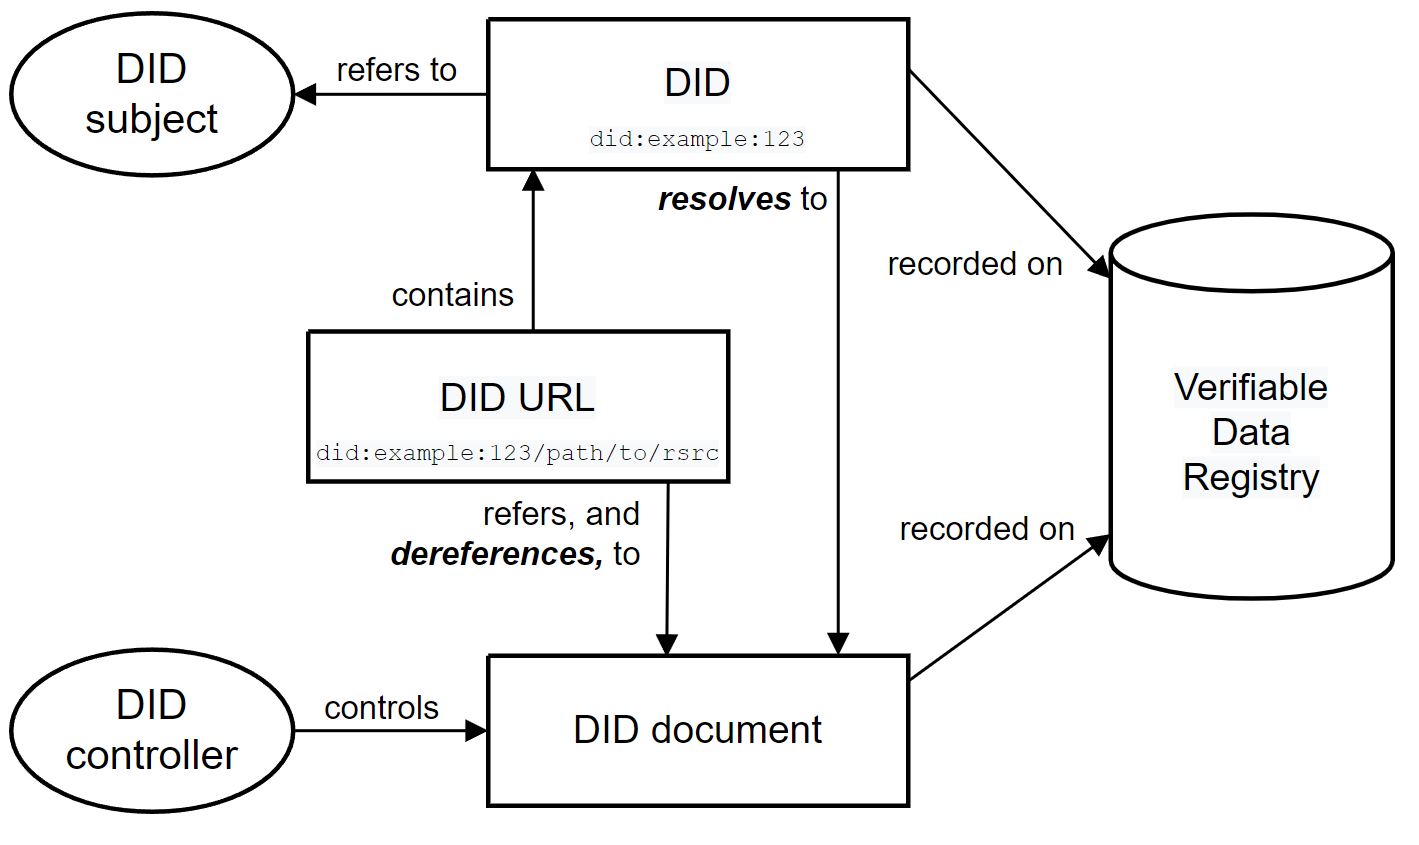
\includegraphics[width=0.75\linewidth]{images/DID_Arquitectura.png}
    \caption{\textit{Arquitectura inicial y relación entre componentes de los \acrshort{DID}s.} Fuente \cite{DID-core}}
    \label{fig:DID}
\end{figure}

Partiendo de esta arquitectura en la que se establecen las bases teóricas del paradigma, podemos extenderla hasta incluir nuevos componentes y mecanismos que permitan la implementación de nuevas utilidades para la gestión de los \acrshort{DID}s y los Documentos DID. 

\begin{itemize}
    \item \textbf{Método DID} (DID Method). \\
    Asociado a una determinada \acrshort{VDR}, define los mecanismos para crear, resolver, actualizar y revocar \acrshort{DID}s al igual que Documentos DID. Es el único componente capaz de modificar los contenidos de el \acrshort{VDR} y por ello deben existir las diferentes implementaciones de las funciones de \underline{Resolución DID} para al menos un Método DID.
    
    \item \textbf{Solucionador DID} (DID Resolver). \\
    Es capaz de generar un Documento DID a partir su correspondiente \acrshort{DID}  mediante la implementación de las funciones de Resolución DID.
    \\
    Un buen ejemplo de ello es la función de deferencia (deference). Mediande ellas se crea el Desreferenciador de URL DID (DID URL Dereferencer), que es un sistema capaz de obtener los recursos a partir de las URL DID.
    \\
\end{itemize}

\begin{figure}[htbp]
    \centering
    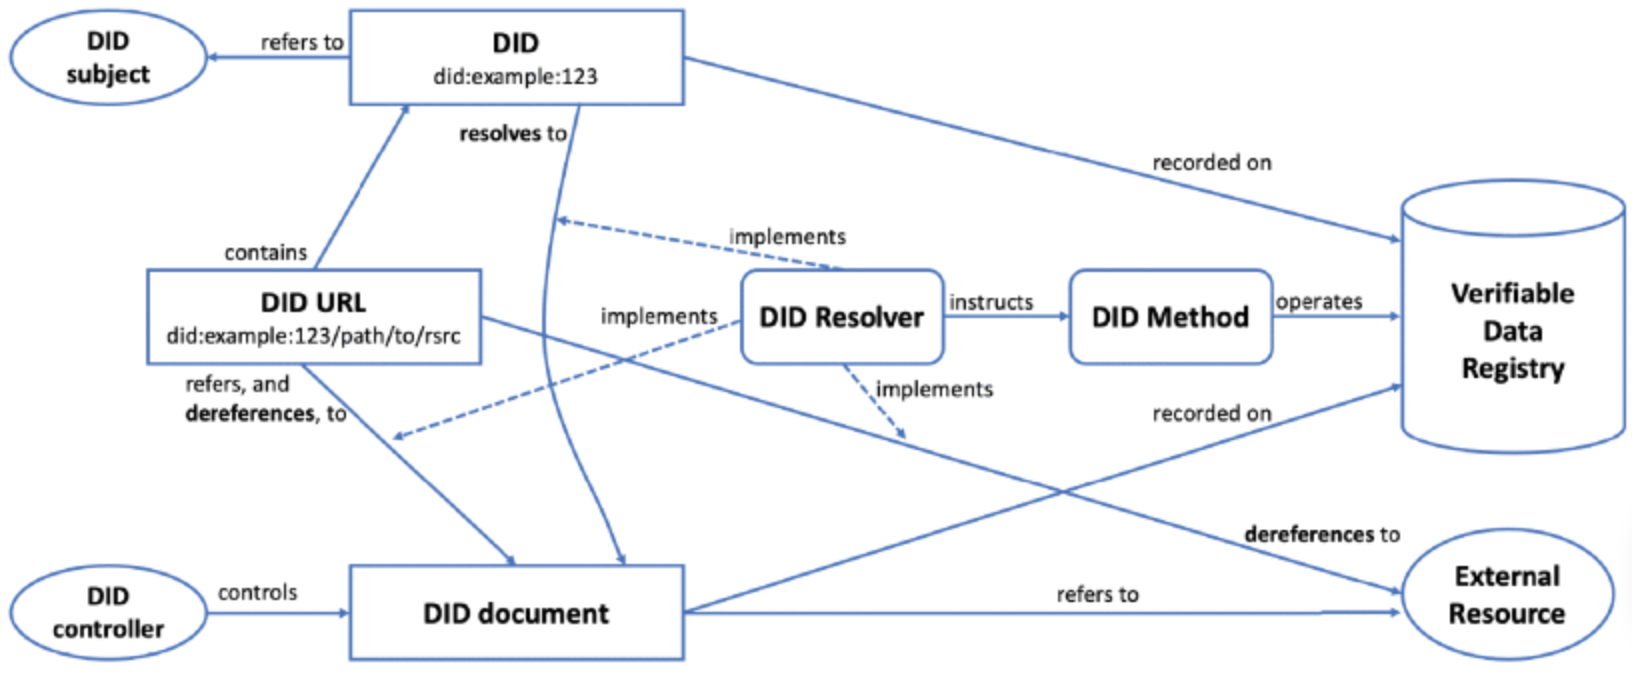
\includegraphics[width=0.85\linewidth]{images/DID_ArquitecturaCompleta.png}
    \caption{\textit{Arquitectura extendida y relación entre componentes de los \acrshort{DID}s.} Fuente \cite{ChallengesSSI}}
    \label{fig:extendedDID}
\end{figure}

Con esta nueva arquitectura se consigue establecer una base técnica funcional que garantiza la identificación de sujetos de manera descentralizada. Sin embargo, el \acrfull{DID} es empleado principalmente como un componente más en sistemas de mayor envergadura , como es el caso de la \acrfull{VC}.


% -------------------------
% Credenciales Verificables
% -------------------------
\newpage
\subsubsection{Credenciales Verificables.}
De igual manera que si de una credencial física se tratase, la \acrfull{VC} permite al usuario identificarse digitalmente ya que contiene su información personal. Sin embargo, mediante el cifrado de estos datos empleando técnicas criptológicas como la \Gls{firma digital}, se consigue que sea ``verificable''. Esto es debido a que cualquier verificador tiene la capacidad de comprobarlas de manera autónoma e independiente \cite{VC-data-model}.  
\\

Como ya se habrá podido intuir, aspectos como los \hyperref[Actores y sus funciones en el paradigma]{actores} que participan en este modelo o los \hyperref[Identificadores Descentralizados]{mecanismos} que permiten la identificación descentralizada son los mismos que han sido descritos con anterioridad. No obstante, se introducen nuevos conceptos como los siguientes:

\begin{itemize}
    \item \textbf{Afirmaciones} (Claims). \\
    Relación entre el sujeto sobre el valor asignado mediante la propiedad que se afirma. Por ejemplo, el autor de este escrito (sujeto) es alumno (propiedad) de la UMA (valor).
    
    \item \textbf{Credenciales} (Credentials). \\
    Conjunto de \underline{afirmaciones} realizados sobre una misma entidad. Opcionalmente puede contener metadatos o pruebas (proofs) y se consideraría ``verificable'' si se realiza un cifrado de estos datos que permita probar criptológicamente quién es el emisor.

    \item \textbf{Presentaciones} (Presentations). \\
    Selección de determinadas \acrshort{VC}s de un mismo Titular para facilitar su transmisión de forma minimalista, consiguiendo así compartir la menor información necesaria.
    \\
    
\end{itemize}

\begin{figure}[htbp]
    \centering
    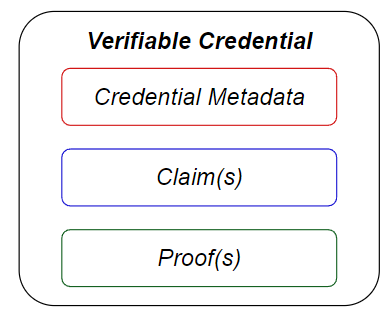
\includegraphics[width=0.3\linewidth]{images/CredencialVerificable.png}
    \caption{\textit{Componentes de una \acrshort{VC}.} Fuente \cite{VC-data-model}}
    \label{fig:VC}
\end{figure}

\end{document}